\documentclass{beamer}

\usepackage[utf8]{inputenc}
\usepackage[T1]{fontenc}
\usepackage[french]{babel}
\usepackage{aeguill}
\usepackage{amsmath}
\usepackage{amsthm}
\usepackage{amssymb}
\usepackage{stmaryrd}
\usepackage{url}
\usepackage{hyperref}
\usepackage{xypic}
%\CompileMatrices
\usepackage{mathpartir}
\usepackage{graphicx}

\renewcommand{\emph}[1]{\alert{#1}}
\renewcommand{\textbf}[1]{{\color{blue} #1}}

\newcommand{\liquidsoap}{Liquidsoap}
\newcommand{\savonet}{Savonet}
\newcommand{\eg}{e.g.~}
\newcommand{\cf}{cf.~}
\newcommand{\letin}[3]{\text{\texttt{let }} #1 = #2 \text{\texttt{ in }} #3}
\newcommand{\univ}[2]{\forall #1.~ #2}
\newcommand{\regle}[1]{\text{\textrm{(#1)}}}
\newcommand{\mabs}[2]{{\color{red}\lambda\{}#1{\color{red}\}.}#2}
\newcommand{\tmabs}[2]{\{#1\}\to #2}
\newcommand{\mapp}[2]{#1{\color{red}\{}#2{\color{red}\}}}
\renewcommand{\vec}[1]{\overrightarrow{#1}}
\newcommand{\TODO}[1]{\textbf{TODO~: }{#1}}
\newcommand{\FV}[1]{\mathcal{FV}(#1)}
\newcommand{\eqdef}{:=}
\newcommand{\interp}[1]{\llbracket{#1}\rrbracket}

%\newtheorem{lemme}{Lemme}
%\newtheorem{theorem}{Theorem}
\newtheorem{proposition}{Proposition}
%\theoremstyle{definition}
%\newtheorem{definition}{Definition}

\author{David Baelde \& Samuel Mimram}
\institute{LIX, \'Ecole Polytechnique, INRIA \&
           PPS, Université Paris VII, CNRS}
\title{De la webradio lambda à la $\lambda$-webdradio}
\date{JFLA, Janvier 2008, Etretat}

\begin{document}

\begin{frame}
  \titlepage
\end{frame}

\newenvironment{ssl}[1]{\begin{frame}\frametitle{#1}}{\end{frame}}
 
% -----------------------------------------------------------------------------

\begin{ssl}{Introduction}
  Quelques aspects du projet Savonet / Liquidsoap,
  un projet de bonne envergure, fruit de la méthodologie fonctionnelle.
  Ici, deux aspects du projet: son coeur, et son interface.
\end{ssl}

\begin{ssl}{\'Etat de l'art}

% \includegraphics[width=10cm,height=5cm]{schema-webradio-inkscape.pdf}

La webradio lambda:
\begin{itemize}
\item
  Outils UNIX, \emph{légers} et \emph{communicants}:
  Ices, EZStream. ou Darkice.
  Diffusion d'un flux à partir d'une \emph{suite de fichiers}
  ou d'une \emph{carte son}.
  % \emph{Interopérable}: interface avec des \emph{outils externes}.
  %On trouve des versions modifiées non maintenues offrant des possibilités 
  %supplémentaires, comme le \emph{crossfading} chez Bide \& Musique.
\item
  Outils professionels:
  Rivendell, Master Control, WinRadio, Open Radio, etc.
  Interface \emph{graphique} intégrant gestion 
  de la playlist, des \emph{transitions}, quelques \emph{traitements audio},
  le décrochage sur \emph{une émission en direct}.
\end{itemize}

La $\lambda$-webradio:
\begin{itemize}
\item Un \emph{modèle de flux audio},
  permettant de définir les opérations souhaitées,
\item un langage de programmation pour composer ces opérations
  et construire sa configuration.
\end{itemize}

\end{ssl}

\begin{ssl}{L'aspect industriel ?}
  LOC, libs pour la gentille communauté, etc.
\end{ssl}

%%%%%%%%%%%%%%%%%%%%%%%%%%%%%%%%%%%%%%%%%%%%%%%%%%%%%%%%%%%%%%%%%%%%%%%%%%%%%%

\begin{ssl}{Graphe des sources}
Une instance de \liquidsoap\ produit un ou plusieurs flux à partir d'un graphe 
constituant sa configuration.

\begin{block}{Un exemple simple}
\[
\xymatrix{
  *+[F]{\mathtt{playlist}}\ar[r]&
  *+[F]{\mathtt{normalize}}\ar[r]&
  *+[F]{\mathtt{output.icecast.vorbis}}\\
}
\]
\end{block}

\begin{block}{Exemple plus complexe}
\[
\xymatrix{
  *+[F]{\mathtt{request.queue}}\ar[r]& *+[F]{\mathtt{mix}}\ar[r]&
    *+[F]{\mathtt{output.icecast}} \\
  *+[F]{\mathtt{playlist}}\ar[ur]\ar[rr] & &
  *+[F]{\mathtt{output.icecast}} \\
}
\]
\end{block}
\end{ssl}

\begin{ssl}{Modèle de flux}
  Qu'est-ce qui sort d'une source ?
  Un flux d'échantillons, regroupés en \emph{pistes},
  qui peut être temporairement \emph{indisponible}.

\begin{block}{Exemple: un \emph{jingle} tous les $3$ morceaux}
\[
\xymatrix{
  *+[F]{\mathtt{playlist("normal.pls")}}\ar[r] &
     *+[F]{\mathtt{random(weights=[1,2])}} \ar[r] & \\
  *+[F]{\mathtt{playlist("jingles.pls")}}\ar[ur] & & \\
}
\]
\end{block}

\begin{block}{Exemple: requêtes d'auditeurs}
\[
\xymatrix{
  *+[F]{\mathtt{request.queue}}\ar[r] &
     *+[F]{\mathtt{fallback}} \ar[r] & \\
  *+[F]{\mathtt{playlist}}\ar[ur] & & \\
}
\]
\end{block}
\end{ssl}

\begin{ssl}{Les transitions}

Pour une écoute agréable, on met en place des \emph{transitions}:
\begin{itemize}
  \item entre pistes d'une même source,
  \item ou quand on passe d'une source à l'autre (e.g. \texttt{fallback}).
\end{itemize}

Types de transitions:
\begin{itemize}
\item Aucune, les pistes sont juxtaposées.
\item Fondu: durée du fondu, en entrée ou en sortie.
\item Fondu croisé (\emph{crossfade}):
 \begin{itemize}
   \item Durées des fondus, durée du recouvrement.
   \item Ajuster les volumes ?
   \item Insérer un jingle ?
 \end{itemize}
\item etc.
\end{itemize}

Solution générique: une transition est une fonction de
$\mathtt{source} \times \mathtt{source} \rightarrow \mathtt{source}$.
\end{ssl}

\begin{ssl}{Exemple typique de transition}
Réalisons un fondu croisé sur la source \texttt{s}:
\begin{semiverbatim}
\begin{enumerate}
\item s = fade.out(duration=3., s)
  \begin{center}
  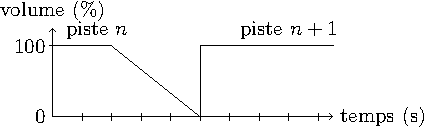
\includegraphics[scale=0.7]{transitions-out.pdf}
  \end{center}
\item s = fade.in(duration=2., s)
  \begin{center}
  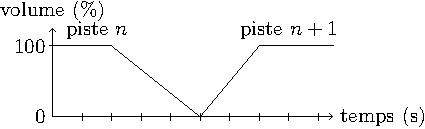
\includegraphics[scale=0.7]{transitions-out-in.pdf}
  \end{center}
\item cross(duration=2., (fun (a,b) -> add([a,b])), s)
  \begin{center}
  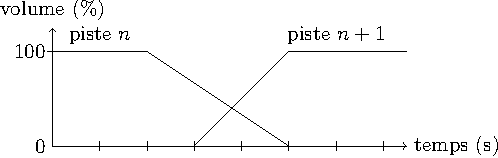
\includegraphics[scale=0.7]{transitions.pdf}
  \end{center}
\end{enumerate}
\end{semiverbatim}
\end{ssl}

\begin{ssl}{Quelques remarques\ldots}
La notion de fonction est désormais étroitement liée à notre modèle.

Passons à la présentation du langage et de son système de types.
\end{ssl}

%%%%%%%%%%%%%%%%%%%%%%%%%%%%%%%%%%%%%%%%%%%%%%%%%%%%%%%%%%%%%%%%%%%%%%%%%%%%%%

\begin{frame}[fragile]
\frametitle{Le langage de script}

Les besoins:
\begin{itemize}
\item Un langage fonctionnel, pour les transitions.
\item Des arguments étiquetés et optionnels pour le confort.
\item Besoin d'analyse statique, intégration de la documentation, simplicité 
  d'utilisation $\Rightarrow$ interpréteur embarqué.
\item Typage statique, inféré $\Rightarrow$ création d'un nouveau langage.
\end{itemize}

\begin{verbatim}
$ liquidsoap -h cross
Generic cross operator, allowing the composition
of the [duration] last seconds of a track with
the beginning of the next track.
Type:
 (?duration:float, ((src, src)->src), src)
 ->src
Parameters:
 duration    :: float (default 5.)
 (unlabeled) :: (src, src)->src    Transition function.
 (unlabeled) :: src
\end{verbatim}
\end{frame}

\begin{frame}[fragile]\frametitle{Les étiquettes d'OCaml}
Les étiquettes d'OCaml sont conçues pour être 
éliminées à la compilation. Garrigue parle d'un \emph{sucre syntaxique typé},
ce qui entraîne quelques limitations:
{\color{blue}\begin{verbatim}
# let app f = f ~a:1 ~b:2 ;;
val app : (a:int -> b:int -> 'a) -> 'a = <fun>
# app (fun ~b ~a -> a+b) ;;
This function should have type a:int -> b:int -> 'a.
\end{verbatim}}

On a besoin d'une multi-application, mais celle-ci ne peut être 
$0$-aire en OCaml (d'où les arguments ineffaçables).
{\color{blue}\begin{verbatim}
# let f ?(a=false) () = a ;;
val f : ?a:bool -> unit -> bool = <fun>
# f () ~a:true ;;
- : bool = true
# (f ()) ~a:true ;;
This expression is not a function, it cannot be applied.
\end{verbatim}}
\end{frame}

\begin{ssl}{Termes}
Les termes sont générés par les constructions suivantes:
\begin{eqnarray*}
  M &::=& v \\
  &|& x \\
  &|& \letin{x}{M}{M} \\
  &|& \lambda \{\ldots, l_i:x_i, \ldots, l_j:x_j=M, \ldots\}.M \\
  &|& M\{l_1=M,\ldots,l_n=M\}
\end{eqnarray*}

%Liaisons: $x$ pour le \verb.let. et les $x_i$ pour la multi-abstraction:
%\begin{eqnarray*}
%  x[M/x] &=& M \\
%  y[M/x] &=& y \text{, si $x\neq y$} \\
%  (\letin{y}{N}{P})[M/x] &=& \letin{y}{N[M/x]}{P[M/x]} \\
%  (\lambda \{ \ldots, l_i:y_i,\ldots,l_j:y_j=N_j, \ldots \}. P)[M/x] &=&
%  \lambda \{ \ldots, l_i:y_i,\ldots, l_j:y_j=N_j[M/x], \ldots \}. (P[M/x])
%  \label{rule:subst-abs} \\
%  (N\{ \ldots, l_i=P_i, \ldots\})[M/x] &=& N[M/x]\{\ldots, l_i=P_i[M/x],\ldots \}
%\end{eqnarray*}

Modulo permutation d'étiquettes distinctes:
\begin{equation*}
  \label{eq:permutation}
 \left.\begin{array}{rcl}
 \lambda \{ \Gamma, l:x, l':x', \Delta \}.M & \equiv &
 \lambda \{ \Gamma, l':x', l:x, \Delta \}.M \\
 \lambda \{ \Gamma, l:x=N, l':x', \Delta \}.M & \equiv &
 \lambda \{ \Gamma, l':x', l:x=N, \Delta \}.M \\
 \lambda \{ \Gamma, l:x=N, l':x'=N', \Delta \}.M & \equiv &
 \lambda \{ \Gamma, l':x'=N', l:x=N, \Delta \}.M
 \end{array}\right\}
 \mbox{ si $l\neq l'$}
\end{equation*}
\end{ssl}

\begin{ssl}{Réduction}
On a trois règles de réduction:
\[
 \letin{x}{M}{N}
   {\color{red}\;\leadsto\;}
   N[M/x]
\]
L'application peut être \emph{partielle},
  si $\Gamma$ est \emph{ineffaçable}:
\[
 (\lambda\{\vec{l_i:x_i,l_j:x_j=M_j},\Gamma\}.M)\{\vec{l_i=N_i}\}
   {\color{red}\;\leadsto\;}
   \lambda\{\Gamma\}.(M[\vec{N_i/x_i}])
  \]
ou \emph{totale} sinon:
\[
(\lambda\{\vec{l_i:x_i,l_j:x_j=P_j},\vec{l'_k:y_k=M_k}\}.M)\{\vec{l_i=N_i}\}
   {\color{red}\;\leadsto\;}
   M[\vec{N_i/x_i},\vec{M_k/y_k}]
 \]

\begin{block}{Exemple}
\begin{itemize}
  \item $F := \mabs{l_1:x,l_2:y={\color{blue}12},l_3:z={\color{blue}13}}{M}$
  \item $\mapp{F}{l_3={\color{blue}3}} \leadsto \mabs{l_1:x,l_2:y={\color{blue}12}}{M[{\color{blue}3}/z]}$
  \item $\mapp{\mapp{F}{l_3={\color{blue}3}}}{l_1={\color{blue}1}} \leadsto M[{\color{blue}1}/x,{\color{blue}12}/y,{\color{blue}3}/z]$
\end{itemize}
\end{block}
\end{ssl}

\begin{ssl}{Typage}
Les types et schémas de types sont sans surprise:
\begin{equation*}
  t \quad::=\quad \iota
  \quad\mathop{|}\quad \alpha
  \quad\mathop{|}\quad
     \{\ldots, l_i:t_i,\ldots, ?l_j:t_j, \ldots\} \rightarrow t
\end{equation*}
\begin{equation*}
  \sigma\quad ::=\quad t
    \quad\mathop{|}\quad \univ{\alpha}{\sigma} \label{tt:univ}
\end{equation*}

On considère naturellement des règles comme:
\[
  \inferrule{%
    \Gamma \vdash M:\{\ldots, l_i:t_i\ldots, ?l_j:t_j,\ldots\}\rightarrow t\\
    \Gamma\vdash N_1:t_1 \\ \cdots \\ \Gamma\vdash N_n:t_n %
  }{%
    \Gamma \vdash M \{ \ldots, l_i=N_i, \ldots, l_j=N_j, \ldots \} : t %
  }{\regle{App}}
\]
ou encore:
\[
  \inferrule{ %
    \Gamma, \ldots, x_i:t_i, \ldots, x_j:t_j, \ldots \vdash M : t
    \\ \cdots \\
    \Gamma\vdash M_j:t_j
    \\ \cdots %
  }{%
    \Gamma\vdash\lambda\{ \ldots, l_i:x_i,\ldots, l_j:x_j=M_j, \ldots \}.M
    : \{ \ldots, l_i:t_i,\ldots, ?l_j:t_j,\ldots \} \rightarrow t}{%
  \regle{Abs}}
\]
\end{ssl}

\begin{ssl}{Sous-typage et application partielle}

La réduction permet l'application partielle. Le système de type, pas encore.
Une fonction de type $\tmabs{l_1:t_1,l_2:t_2}{t}$
doit pouvoir être considérée comme une fonction de type
$\tmabs{l_1:t_1}{\tmabs{l_2:t_2}{t}}$.

\[
\inferrule{\mbox{$\Delta$ ineffaçable}}{
  \{ \Gamma, \Delta \}\rightarrow t {\color{red}\leq}
       \{\Gamma\}\rightarrow\{\Delta\}\rightarrow t
}
\qquad
\inferrule{\mbox{$\Delta$ effaçable}}{
  \{ \Gamma, \Delta \}\rightarrow t {\color{red}\leq} \{\Gamma\}\rightarrow t
}
\]

Quelques équations invalides:
\begin{itemize}
\item $
\tmabs{l_1:t_1}{\tmabs{l_2:t_2}{t}}
{\color{red}\not\leq}
\tmabs{l_1:t_1,l_2:t_2}{t}
$
\item $\tmabs{\Gamma,?l:t,\Delta}{t'} {\color{red}\not\leq}
  \tmabs{\Gamma,l:t,\Delta}{t'}$
\end{itemize}
\end{ssl}

\begin{ssl}{Inférence}
Pas de type principal, mais on peut plonger

En pratique: inférence limitée aux cas simples.
\end{ssl}

%%%%%%%%%%%%%%%%%%%%%%%%%%%%%%%%%%%%%%%%%%%%%%%%%%%%%%%%%%%%%%%%%%%%%%%%%%%%%%

\begin{ssl}{Conclusion}
\begin{block}{Contributions}
\begin{itemize}
\item Vulgarisation:
  \begin{itemize}
  \item Une application \emph{OCaml} de plus \emph{pour la ``vraie vie''},
  \item un langage fonctionnel, avec types statiques inférés,
    pour l'utilisateur lambda.
  \end{itemize}
\item Une variante originale du $\lambda$-calcul.
\item Beaucoup de composants re-utilisables.
\end{itemize}
\end{block}
\begin{block}{Travaux futurs}
\begin{itemize}
\item Format de flux hétérogènes.
\item vérification statique de l'\emph{exclusivité}
  requise par certains opérateur, de la \emph{vivacité} d'un flux.
\item Variante du langage avec application partielle explicitée,
  et inférence complète ?
\item Lien avec nos activités de recherche: vérification formelle.
\end{itemize}
\end{block}
\end{ssl}

\end{document}
